% Estas slides tienen que abrirse con el programa pdfpc que soporta videos embebidos. Para los videos se requiere ubuntu-restricted-extras. El comando es: pdfpc -g slides.pdf

% compress: Encabezado muestra solo la section actual
\documentclass[compress]{beamer}
\mode<presentation>

\usetheme{Copenhagen}
\useoutertheme{taihu}
%\useinnertheme{rectangles}

% Itemize configuration
\setbeamertemplate{itemize item}[rectangle]
\setbeamertemplate{itemize subitem}[circle]
\setbeamertemplate{itemize subsubitem}[triangle]

%\setbeamertemplate{navigation symbols}{} % Remover símbolos de navegación
\usefonttheme[onlymath]{serif} % Símbolos matemáticos en Serif

\setbeamertemplate{blocks}[rounded] % Block corners rounded
\setbeamercolor{block body}{bg=blue!12,fg=black} % Color of blocks

\usepackage{pdfpc-commands} % pdfpc movie commands
\usepackage[utf8]{inputenc}
\usepackage[spanish]{babel}
\usepackage[binary-units=true]{siunitx} % Para manejar las unidades
\usepackage{multirow}
\usepackage{multimedia}
\usepackage{graphicx}
\usepackage{xcolor}
\usepackage{booktabs} % \toprule

% Elimina la palabra 'Figura' del caption
\usepackage[caption=false]{subfig}
\setbeamertemplate{caption}{\raggedright\insertcaption\par}
\captionsetup[subfigure]{labelformat=empty} % Remover índice del caption de la subfigura

\usepackage{import} % Para el comando import (se usa para pdf_tex)

% Para notas personales en el pdfpc
\usepackage{pdfpcnotes}

\AtBeginSection[]
{
   \begin{frame}
       \frametitle{Índice}
       \tableofcontents[currentsection]
   \end{frame}
}

\usepackage{amsmath}
\usepackage{amssymb}
\usepackage{amsopn}

% math
\renewcommand{\vec}[1]{\boldsymbol{\mathbf{#1}}}
\newcommand{\norm}[1]{\left\lVert#1\right\rVert}

% Declare arg max and arg min functionss
\DeclareMathOperator*{\argmax}{arg\,max}
\DeclareMathOperator*{\argmin}{arg\,min}

% Homogeneous decoration function
\newcommand{\homo}[1]{\dot{#1}}

% Declare projection as math function
\DeclareMathOperator{\proj}{proj}
\DeclareMathOperator{\disp}{disp}
\newcommand{\worldCoordSystem}{\mathrm{w}}
\newcommand{\cameraCoordSystem}{\mathrm{c}}
\newcommand{\point}{\vec{x}}
\newcommand{\worldPoint}{\point^{\mathrm{w}}}
\newcommand{\homoWorldPoint}{\homo{\point}^{\mathrm{w}}}
\newcommand{\cameraPoint}{\point^{\mathrm{c}}}
\newcommand{\hatCameraPoint}{\hat{\point}^{\mathrm{c}}}
\newcommand{\homoCameraPoint}{\homo{\point}^{\mathrm{c}}}
\newcommand{\measurement}{\vec{z}}
\newcommand{\prediction}{\hat{\vec{z}}}
\newcommand{\imagePoint}{\vec{u}}
\newcommand{\seMatrix}{\vec{E}}
\newcommand{\rotation}{\vec{R}}
\newcommand{\translation}{\vec{t}}
\newcommand{\intrinsicMatrix}{\vec{K}}
\newcommand{\principalPoint}{\vec{c}}
\newcommand{\reprojectionError}{u}
\newcommand{\projectionMatrix}{\vec{P}}
\newcommand{\cameraCenter}{\vec{o}}


% Dense Map
\newcommand{\current}{\mathrm{current}}
\newcommand{\previous}{\mathrm{previous}}
\newcommand{\fusion}{\mathrm{fusion}}
\newcommand{\inverseDepth}{\rho}
\newcommand{\plane}{\boldsymbol{\pi}}
\newcommand{\reference}{ref}


% scaled operators and letters to fancy view
\newcommand{\sminus}{\scalebox{0.5}[1.0]{$-$}}
\newcommand{\splus}{\scalebox{0.6}[0.6]{$+$}}
\newcommand{\curr}{c}
\newcommand{\sind}[1]{\scalebox{0.6}[0.6]{$#1$}}
\newcommand{\ind}[1]{\scalebox{0.7}[0.7]{$#1$}}

\newcommand{\keyframe}{\vec{K}}
\newcommand{\pointCloud}{\mathcal P}
\newcommand{\groundTruth}[1]{{#1}^{*}}

\newcommand{\update}[1]{\hat{#1}}

\newcommand{\position}{\vec{p}}
\newcommand{\map}{M}

\newcommand{\baseline}{b}
\newcommand{\focalDistance}{f}
\newcommand{\disparityMap}{\mathcal D}
\newcommand{\camera}{c}
\newcommand{\ray}{n}


\author{\textbf{Autor:} D'Alessandro, Ariel \\ \textbf{Director:} Pire, Taihú \and \textbf{Co-director}: Baravalle, Rodrigo}

\setbeamerfont{title}{size=\large}
\title{Mapeo denso en tiempo real sobre sistemas SLAM basados en visión estéreo}

\institute{FCEIA - UNR}
\date{\scriptsize{Diciembre 22, 2017}}

\begin{document}

\frame{\titlepage}

\begin{frame}
\frametitle{Índice}
\tableofcontents
\end{frame}

\section{Introducción}


\begin{frame}
\frametitle{Motivación}

\begin{block}{Objetivo a desarrollar}
Método de reconstrucción 3D o mapeo denso en tiempo real sobre sistemas de localización y mapeo simultáneo (SLAM) basado en visión estéreo.
\end{block}

\end{frame}


\begin{frame}
\frametitle{Reconstrucción 3D}

\pnote{* Reconstrucción 3D: Proceso mediante el cual se captura y representa la forma y apariencia de entornos u objetos presentes en la realidad. Diseño asistido por computadora, imágenes médicas, realidad virtual y aumentada, robótica movil, entre otros.}

\pnote{* Uno de los principales problemas presentes en aplicaciones relativas a robots autónomos móviles consiste en el planeamiento de una trayectoria segura hacia determinados objetivos, mientras el robot se desplaza a través de un entorno potencialmente desconocido.}

\pnote{* Para esto, resulta necesario contar con una representación del ambiente que se está transitando (mapa) y la ubicación del robot dentro del mismo (SLAM - slide siguiente).}

\pnote{* El mapa debe ser suficientemente detallado (denso) para que el robot pueda realizar un planeamiento seguro, evitando posibles obstáculos.}

\begin{figure}[!htb]
	\centering
	\subfloat[]{\includegraphics[width=0.30\columnwidth]{./introduction/3d-skull.jpg}}%
	\hfill
	\subfloat[]{\includegraphics[width=0.30\columnwidth]{./introduction/3d-dinosaur.jpg}}%
	\hfill
	\centering
	\subfloat[]{\includegraphics[width=0.40\columnwidth]{./introduction/3d-indoor.jpg}}%
	\hfill
	\\
	\centering
	\subfloat[]{\includegraphics[width=0.70\columnwidth]{./introduction/3d-building.png}}%
	\hfill
\end{figure}

\end{frame}


\begin{frame}
\frametitle{SLAM - Simultaneous Localisation and Mapping}

\pnote{* A partir de la detección y seguimiento de marcas naturales del ambiente (landmarks), los sistemas de SLAM pueden estimar tanto la posición del robot como la ubicación de estas marcas en el entorno. El mapa es construído incrementalmente con las posiciones estimadas de dichas marcas, las cuales son ajustadas a lo largo de la trayectoria a medida que son observadas.}

\begin{itemize}
\item Construir incrementalmente un mapa del entorno.
\item Determinar su posición y orientación en el mismo.
\end{itemize}

\begin{figure}[!htb]
	\centering
	\subfloat[]{\includegraphics[width=0.50\columnwidth]{./introduction/slam-landmarks.pdf}}%
	\hfill
\end{figure}

\end{frame}


\begin{frame}
\frametitle{SLAM Visual - Cámaras}

\pnote{* Cámaras: rica información de la escena. Ventajas: bajo costo, menor consumo energético en comparación con otros sensores, como lásers, portabilidad y alta disponibilidad en dispositivos móviles. Son sensores pasivos por lo que no interferen con otros sensores y pueden utilizarse en entornos interiores, donde el uso de GPS puede verse imposibilitado. Asímismo, son menos restrictivos que los encoders, los cuales se encuentran limitados a robots terrestres y resultan imprecisos en terrenos irregulares.}

\begin{itemize}
\item Bajo costo.
\item Bajo consumo energético.
\item Alta disponibilidad en dispositivos móviles.
\item Sensores pasivos.
\item Apto entornos interiores.
\item Apto terrenos irregulares.
\end{itemize}

\end{frame}


\begin{frame}
\frametitle{SLAM Visual - Cámaras estéreo}

\pnote{* Cámaras estéreo: Existen dos enfoques predominantes en los sistemas de SLAM basados en cámaras, denominados monocular y estéreo. Los sistemas de SLAM visual estéreo proveen información sobre la profundidad de los píxeles mediante una única observación, lo cual requiere mayor número de cómputos en el caso monocular.}

\begin{figure}[!htb]
	\centering
	\subfloat[]{\includegraphics[width=0.45\columnwidth]{./introduction/camera-stereo-old.jpg}}%
	\hfill
	\centering
	\subfloat[]{\includegraphics[width=0.45\columnwidth]{./introduction/camera-stereo-new.jpg}}%
	\hfill
\end{figure}

\end{frame}
\section{Cámaras como sensores}


\begin{frame}
\frametitle{Modelo de cámara}

\begin{block}{Definición - Cámara}
Una cámara es definida matemáticamente como una correspondencia entre el mundo 3D y una imagen 2D. Es decir, un mapeo entre puntos del mundo 3D $\point$ y puntos de la imagen $\imagePoint$:
\begin{equation}
\point=\begin{bmatrix}x\\
y\\
z
\end{bmatrix}\longmapsto
\imagePoint=\begin{bmatrix}u\\
v
\end{bmatrix}
\end{equation}
\end{block}

\end{frame}


\begin{frame}
\frametitle{Modelo de cámara pinhole}

\pnote{* Rayo principal o eje principal de la cámara: rayo que se origina en el centro focal \cameraCenter y es perpendicular al plano de la imagen.}

\pnote{* Punto principal: el punto donde este rayo intersecta al plano de la imagen es denominado.}

\begin{block}{Cámara pinhole}
El punto de la imagen $\imagePoint=\begin{bmatrix}u & v\end{bmatrix}^{\top}$ es determinado como la intersección entre el \emph{plano de la imagen} y el rayo que une el punto del mundo 3D $\point=\begin{bmatrix}x & y & z\end{bmatrix}^{\top}$ con el \emph{centro focal} $\cameraCenter$ de la cámara.
\end{block}

\begin{figure}[!htb]
	\centering
	\subfloat[]{\includegraphics[width=0.5\columnwidth]{./cameras/pinhole_camera_model.pdf}}%
	\hfill
\end{figure}

\end{frame}


\begin{frame}
\frametitle{Modelo de cámara pinhole}

\pnote{* Proyección central: Utilizando la propiedad de semejanza de triángulos, el punto 3D es mapeado al punto en el plano de la imagen.}

\begin{block}{Proyección central}
Asumiendo el centro focal en el origen de coordenadas y el plano de la imagen $Z=f$:

\begin{equation}
\begin{bmatrix}x\\
y\\
z
\end{bmatrix}\longmapsto\begin{bmatrix}fx/z\\
fy/z
\end{bmatrix}
\end{equation}

\end{block}

\begin{figure}[!htb]
	\centering
	\subfloat[]{\includegraphics[width=0.5\columnwidth]{./cameras/pinhole_camera_model.pdf}}%
	\hfill
	\centering
	\subfloat[]{\includegraphics[width=0.5\columnwidth]{./cameras/pinhole_camera_model2.pdf}}%
	\hfill
\end{figure}

\end{frame}


\begin{frame}
\frametitle{Modelo de cámara pinhole}

\pnote{* Lo anterior asume que el origen de coordenadas del plano de la imagen se encuentra en el punto principal. En la práctica, esto no siempre se cumple.}

\pnote{* Explicar representación en coordenadas homogéneas.}

Siendo $\begin{bmatrix}c_{u} & c_{v}\end{bmatrix}^{\top}$ la posición del punto principal.
\begin{equation}
\begin{bmatrix}x\\
y\\
z
\end{bmatrix}\longmapsto\begin{bmatrix}fx/z+c_{u}\\
fy/z+c_{v}
\end{bmatrix}
\end{equation}

En coordenadas homogéneas:

\begin{equation}
\begin{bmatrix}x\\
y\\
z\\
1
\end{bmatrix}\longmapsto\begin{bmatrix}fx+zc_{u}\\
fy+zc_{v}\\
z
\end{bmatrix}=\begin{bmatrix}f &  & c_{u} & 0\\
 & f & c_{v} & 0\\
 &  & 1 & 0
\end{bmatrix}\begin{bmatrix}x\\
y\\
z\\
1
\end{bmatrix}
\end{equation}

\begin{block}{Matriz de calibración intrínseca $\intrinsicMatrix$}
\begin{equation}
\intrinsicMatrix=\begin{bmatrix}f & 0 & c_{u}\\
0 & f & c_{v}\\
0 & 0 & 1
\end{bmatrix}
\end{equation}
\begin{equation}
\homo{\imagePoint}=\intrinsicMatrix\begin{bmatrix}\vec{{I}} & \vec{{0}}\end{bmatrix}\homo{\point}
\end{equation}
\end{block}

\end{frame}


\begin{frame}
\frametitle{Modelo de cámara pinhole}

\pnote{* Las ecuaciones anteriores deben extenderse agregando la transformación existente entre los sistemas de coordenadas de la cámara y el mundo.}

\pnote{* R es una matriz de rotación y t un vector de traslación.}

Puntos expresados en referencia al sistema de coordenadas del \textit{mundo}. La cámara no se encuentra necesariamente ubicada en el centro de este.

\begin{figure}[!htb]
	\centering
	\subfloat[]{\includegraphics[width=0.4\columnwidth]{./cameras/camera_coord_system.pdf}}%
	\hfill
\end{figure}

\begin{block}{}
\begin{equation}
\homoCameraPoint=\begin{bmatrix}\rotation & \translation\\
0 & 1
\end{bmatrix}\begin{bmatrix}x\\
y\\
z\\
1
\end{bmatrix}=\seMatrix^{\mathrm{c}\mathrm{w}}\homoWorldPoint\;.
\end{equation}
\end{block}

\end{frame}


\begin{frame}
\frametitle{Modelo de cámara pinhole}

De esta manera, es posible proyectar cualquier punto 3D
$\homoWorldPoint$ en el sistema de coordenadas del mundo al correspondiente
punto $\homo{\imagePoint}$ en el plano de la imagen mediante:

\begin{block}{Matriz de proyección \textmd{$\projectionMatrix$}}
\begin{equation}
\projectionMatrix=\intrinsicMatrix\begin{bmatrix}\rotation & \translation\end{bmatrix}
\end{equation}
\begin{equation}
\homo{\imagePoint}=\projectionMatrix\homoWorldPoint
\end{equation}
\end{block}

\end{frame}


\begin{frame}
\frametitle{Modelo de cámara estéreo}

\begin{block}{Geometría epipolar}

\pnote{* La geometría proyectiva intrínseca entre dos cámaras es conocida como geometría epipolar.}

\pnote{* Esta es independiente de la escena observada y depende únicamente de los parámetros internos geometría epipolar y las posiciones relativas de las cámaras involucradas.}

Cualquier punto 3D $\point$ en el espacio, sus proyecciones $\imagePoint$ y $\imagePoint^{\prime}$ en los planos de las imágenes y los centros focales de las cámaras, pertenecen a un mismo plano $\vec{\pi}$.
De manera análoga, los rayos re-proyectados desde $\imagePoint$ y $\imagePoint^{\prime}$ se intersectan en $\point$, son coplanares y yacen sobre $\vec{\pi}$.
\end{block}

\begin{figure}[!htb]
	\centering
	\subfloat[]{\includegraphics[width=0.5\columnwidth]{./cameras/pencil_of_planes.pdf}}%
	\hfill
	\centering
	\subfloat[]{\includegraphics[width=0.5\columnwidth]{./cameras/epipolar_plane.pdf}}%
	\hfill
\end{figure}
\end{frame}


\begin{frame}
\frametitle{Modelo de cámara estéreo}

\pnote{* La búsqueda del correspondiente al punto u no necesita cubrir el plano de la imagen completo sino que puede restringirse a la línea epipolar l.}

\pnote{* La línea epipolar es generada por la proyección del rayo, re-proyectado desde u, sobre el plano focal de la segunda imagen.}

Búsqueda de correspondencias sobre la línea epipolar.

\begin{figure}[!htb]
	\centering
	\subfloat[]{\includegraphics[width=0.5\columnwidth]{./cameras/epipolar_line.pdf}}%
	\hfill
\end{figure}
\end{frame}


\begin{frame}
\frametitle{Rectificación estéreo}

\pnote{* Luego de aplicar rectificación estéreo, la búsqueda de correspondencias entre las imágenes es reducida a una búsqueda unidimensional, sobre la misma fila.}

\begin{itemize}
\item Proyectar el par de imágenes estéreo sobre un plano de imagen común.
\item Los puntos correspondientes se encuentren alineados en la misma fila.
\end{itemize}

\begin{figure}[!htb]
	\centering
	\subfloat[]{\includegraphics[width=0.6\columnwidth]{./cameras/stereo_rectification.pdf}}%
	\hfill
\end{figure}
\end{frame}


\begin{frame}
\frametitle{Rectificación estéreo}

\pnote{* Rectificación estéreo sobre un par de imágenes del Dataset Level 7 [32]. (a) Par de imágenes estéreo original provisto por la cámara estéreo.}
\pnote{* (b) El par de imágenes estéreo luego de ser rectificadas. Las líneas rojas asocian algunos puntos correspondientes entre ambas imágenes. Notar que estos puntos se encuentran en la misma fila en ambas imágenes.}

\begin{figure}[!htb]
	\centering
	\subfloat[]{\includegraphics[width=0.6\columnwidth]{./cameras/no_rectified_stereo_images.png}}%
	\hfill
	\\
	\centering
	\subfloat[]{\includegraphics[width=0.6\columnwidth]{./cameras/rectified_stereo_images.png}}%
	\hfill
\end{figure}
\end{frame}


\begin{frame}
\frametitle{Triangulación estéreo}

\pnote{* Sea x = x y z un punto 3D cuyas coordenadas son desconocidas. Conociendo las proyecciones correspondientes, la posición del punto x puede ser derivada.}

\pnote{* Aplicando la propiedad de triángulos semejantes entre el triángulo de línea negra punteada y el triángulo de línea roja en la Figura, la siguiente ecuación puede ser formulada.}

Proyecciones correspondientes $\imagePoint_{l}=\begin{bmatrix}u_{l} & v_{l}\end{bmatrix}$ y $\imagePoint_{r}=\begin{bmatrix}u_{r} & v_{r}\end{bmatrix}$ sobre los planos focales de la imagen izquierda y derecha respectivamente,
la posición del punto $\point$ puede ser derivada.

\begin{equation}
\frac{b}{z}=\frac{(b+u_{r})-u_{l}}{z-f}
\end{equation}

\begin{figure}[!htb]
	\centering
	\subfloat[]{\includegraphics[width=0.5\columnwidth]{./cameras/stereo_triangulation.pdf}}%
	\hfill
	\centering
	\subfloat[]{\includegraphics[width=0.5\columnwidth]{./cameras/stereo_triangulation2.pdf}}%
	\hfill
\end{figure}
\end{frame}


\begin{frame}
\frametitle{Triangulación estéreo}

\pnote{* De la misma manera, utilizando propiedad de triángulos semejantes nuevamente sobre la Figura, se obtienen las restantes ecuaciones.}

\begin{equation}
\frac{x}{z}=\frac{u_{l}-c_{u}}{f}\qquad\frac{y}{z}=\frac{v_{l}-c_{v}}{f}
\end{equation}

\begin{equation}
\begin{aligned}x=\frac{(u_{l}-c_{u})z}{f}\;\qquad
y=\frac{(v_{l}-c_{v})z}{f}\;\qquad
z=\frac{bf}{u_{l}-u_{r}}\;
\end{aligned}
\end{equation}

\begin{figure}[!htb]
	\centering
	\subfloat[]{\includegraphics[width=0.5\columnwidth]{./cameras/stereo_triangulation.pdf}}%
	\hfill
	\centering
	\subfloat[]{\includegraphics[width=0.5\columnwidth]{./cameras/stereo_triangulation2.pdf}}%
	\hfill
\end{figure}
\end{frame}


\begin{frame}
\frametitle{Disparidad}

\pnote{* Cuando el valor de disparidad $d$ es cercano a $0$, pequeñas diferencias de disparidad producen un gran cambio en la profundidad del punto. En consecuencia, la reconstrucción 3D del ambiente mediante cámaras estéreo es más precisa para puntos cercanos a la cámara.}

\begin{block}{Definición - Disparidad}
La disparidad $d$ es definida como la distancia existente entre las proyecciones de las diferentes cámaras.
\begin{equation}
d=u_{l}-u_{r}=\frac{bf}{z}
\end{equation}
\end{block}

\textbf{Nota}: la profundidad $z$ es inversamente proporcional a la disparidad $d$.

\end{frame}
\section{Método}

\begin{frame}
	\frametitle{Dense S-PTAM}
	\begin{figure}[htb]
		\centering
		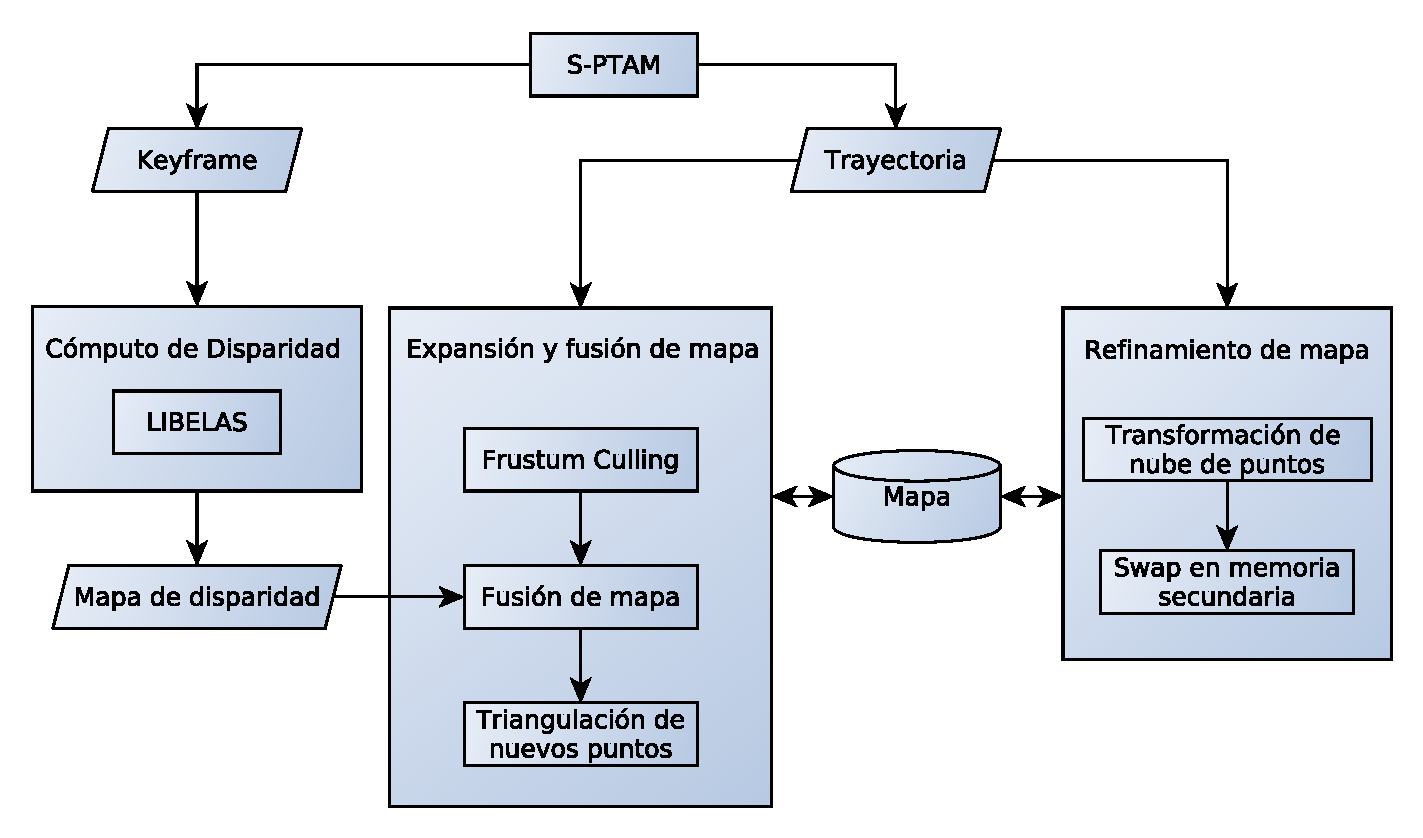
\includegraphics[width=0.8\columnwidth]{images/dense_diagram.pdf}
	\end{figure}
\end{frame}

\begin{frame}
	\frametitle{Expansión y fusión de mapa}
	\begin{figure}[htb]
		\centering
		\includegraphics[width=\columnwidth]{images/map_fusion.pdf}
	\end{figure}
	
	\begin{equation*}
		\point_{\mathrm{\fusion}} = \dfrac{1}{\inverseDepth_\mathrm{\fusion}} \dfrac{\point_{\mathrm{\current}}}{\norm{\point_{\mathrm{\current}}}}
		\quad \text{donde} \quad 
		\inverseDepth_{\fusion} = \dfrac{\inverseDepth_{\current} + \inverseDepth_{\previous}}{2}
	\end{equation*}
\end{frame}

\input{experiments/experiments.tex}
\section{Conclusiones}

\begin{frame}
	\frametitle{Conclusiones}
	\begin{itemize}
		\item Sistema de SLAM capaz de generar un \textbf{mapa local denso} en \textbf{tiempo real}
        \item La precisión es útil para tareas de \textbf{navegación}
        \item Funciona incluso en trajectorias de grandes dimensiones
        \item Evaluado en datasets públicos: KITTI (outdoors) y Tsukuba (indoors)
	    \item Código open-source en ROS (GPLv3)
	    \url{https://github.com/CIFASIS/dense-sptam}
	\end{itemize}
\end{frame}

\begin{frame}
	\frametitle{Trabajo Futuro}
	\begin{itemize}
		\item Tomar ventaja del módulo de cierre de ciclos (\emph{Loop Closure})
		\item Utilizar información de apariencia para el matching de puntos
		\item Aproximar con planos nubes de puntos referentes a superficies planas
	\end{itemize}
\end{frame}

\section*{}

\begin{frame}
	\centering
	\Large{Muchísimas gracias!}
	
	\pause{Preguntas?}
	
	\vspace{2cm}
	Contacto: {\tt pire@cifasis-conicet.gov.ar}
\end{frame}

\end{document}